\subsection{Heap-Sort Algorithm:}

For the following algorithm we create a {\itshape Class} with the name of the algorithm, in its constructor will receive as parameters only the list to sort, this list has the name of {\itshape dimensions} as we can see in line 3, in line 4 the program corroborates that the length of {\itshape dimensions} it's bigger than 1, in case that do not accomplish the condition then the program stops running because there is no need of sorting, otherwise the program continues running and in line 6 stores in a instance of the class the length of {\itshape dimensions}, this two variables are going to be used along the execution. \hfill \break

Heap sort is a comparison sorting technique based on Binary Heap data structure. It is similar to selection sort where we first find the maximum element and place the maximum element at the end. We repeat the same process for the remaining element. In line 9 it's written the algorithm that will {\itshape heapify} the root of the tree, this algorithm assumes that the binaries trees rooted at LEFT ( j ) and RIGHT ( j ) are max heaps, but {\itshape dimensions [ j ]} might be smaller than its children, thus violating the max-heap property. Lets the value at {\itshape dimensions [ j ]} 'float down' in the max-heap so that the sub-tree rooted at index {\itshape j} obeys the max-heap property. \hfill \break

\begin{lstlisting}
class Heapsort:
    # Class constructor.
    def __init__ ( self, dimensions ):
        assert len ( dimensions ) > 1
        self.dimensions = dimensions
        self.n = len ( dimensions )

    # Heapify subtree rooted at index j.
    def heapify ( self, i, j ):
        right = 2 * j + 2
        left = 2 * j + 1
        largest = j
        # Verify if the left child exist and if it's greater than the root.
        if ( left < i and self.dimensions [ j ] < self.dimensions [ left ] ):
            largest = left
        # Verify if the right child exist and if it's greater than the root.
        if ( right < i and self.dimensions [ largest ] < self.dimensions [ right ] ):
            largest = right
        # Change the root if it's needed.
        if ( largest != j ):
            aux = self.dimensions [ j ]
            self.dimensions [ j ] = self.dimensions [ largest ]
            self.dimensions [ largest ] = aux
            # Heapify the root.
            self.heapify ( i, largest )

    # Heapsort algorithm.
    def heapsort ( self ):
        # Build the max heap.
        for i in range ( self.n, -1, -1 ):
            self.heapify ( self.n, i )
        # Extract the elements one by one.
        for i in range ( ( self.n - 1 ), 0, -1 ):
            aux = self.dimensions [ i ]
            self.dimensions [ i ] = self.dimensions [ 0 ]
            self.dimensions [ 0 ] = aux
            self.heapify ( i, 0 )
\end{lstlisting} \hfill \break

Figure 3.1.0 illustrates the action of the method {\itshape heapify}. At each step, the largest of the elements {\itshape dimensions [ j ]}, {\itshape dimensions [ left ]} and {\itshape dimensions [ right ]} is determined, and its index is stored in largest as we can see in lines 14 - 18. If {\itshape dimensions [ j ]} is largest, then the sub-tree rooted at node {\itshape j} is already a max-heap and the procedure terminates. Otherwise, one of the two children has the largest element, and {\itshape dimensions [ j ]} is swapped with {\itshape dimensions [ largest ]} as we can see from lines 20 - 23, which causes node {\itshape j} and its children to satisfy the max-heap property. The node indexed by largest, however, now has the original value {\itshape dimensions [ j ]}, and thus the sub-tree rooted at largest might violate the max-heap property. Consequently, in line 25 we will call recursively {\itshape heapify} on that sub-tree.

\begin{figure}[H]
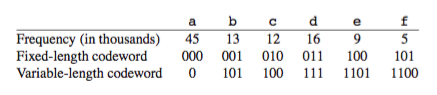
\includegraphics[width = 16.5cm, height = 10cm]{1.png}
{\centering \linebreak \linebreak \small Figure 3.1.0: The action of {\itshape heapify ( 10, 2 )}, where 10 it's the heap size. {\bfseries (a)} The initial configuration, with {\itshape dimensions [ 2 ]} at node {\itshape i = 2} violating the max-heap property since it is not larger than both children. The max-heap property is restored for node 2 in {\bfseries (b)} by exchanging {\itshape dimensions [ 2 ]} with {\itshape dimensions [ 4 ]}, which destroys the max-heap property for node 4. The recursive call {\itshape heapify ( 10, 4 )} now has {\itshape i = 4}. After swapping {\itshape dimensions [ 4 ]} with {\itshape dimensions [ 9 ]}, as shown in {\bfseries (c)}, node 4 is fixed up, and the recursive call {\itshape heapify ( 10, 9 )} yields no further change to the data structure.}
\end{figure} \hfill

In lines 30 - 31 the algorithm will build the {\itshape max-heap} by using the algorithm {\itshape heapify} as we can see in line 31. The procedure to build a {\itshape max-heap} goes through the remaining nodes of the tree and runs {\itshape heapify} on each one. Figure 3.1.1 shows an example of building a {\itshape max-heap}. \hfill \break

\begin{figure}[H]
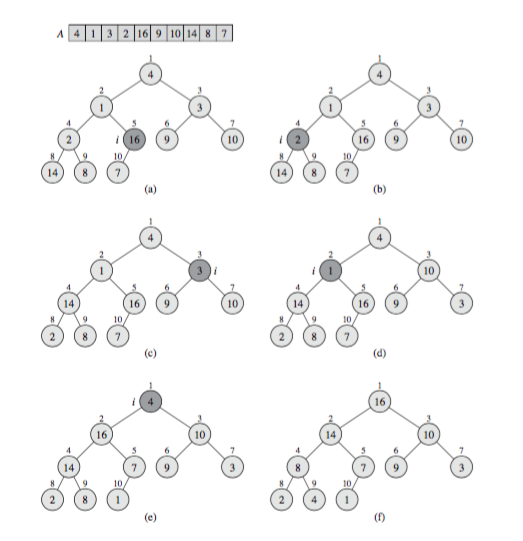
\includegraphics[width = 16.5cm, height = 8cm]{0.png}
{\centering \linebreak \linebreak \small Figure 3.1.1: The operation of building a {\itshape max-heap}, showing the data structure before the call to {\itshape heapify} in line 31. {\bfseries (a)} A 10-element input array {\bfseries A} and the binary tree it represents. The figure shows that the loop index {\itshape i} refers to node 5 before the call {\itshape heapify ( 10, i )}. {\bfseries (b)} The data structure that results. The loop index {\itshape i} for the next iteration refers to node 4. {\bfseries (c)-(e)} Subsequent iterations of the {\bfseries loop} in line 30. Observe that whenever {\itshape heapify} is called on a node, the two sub-trees of that node are both {\itshape max-heap}. {\bfseries (f)} Building the max heap process it's finished.}
\end{figure} \hfill \break

After building the {\itshape max-heap} the 'really' {\itshape Heap-Sort} algorithm begins. Since the maximum element of the array is stored at the root {\itshape dimensions [ 0 ]}, we can put it into its correct final position by exchanging it with {\itshape dimensions [ n ]}. If we now discard node {\bfseries n} from the heap and we can do so by simply decreasing the {\itshape heap-size} we observe that the children of the root remain {\itshape max-heaps}, but the new root element might violate the {\itshape max-heap} property. All we need to do to restore the {\itshape max-heap} property, however, is call {\itshape heapify ( i, 0 )} as we can see in line 37 which leaves a {\itshape max-heap} in {\itshape dimensions [ 1 ... n - 1 ]}. The {\itshape Heap-Sort} algorithm then repeats this process for the {\itshape max-heap} of size {\itshape n - 1} down to a heap of size {\itshape 1}. \hfill \break

Figure 3.1.2 shows an example of the operation of this algorithm after building the {\itshape max-heap}. \hfill \break 

\begin{figure}[H]
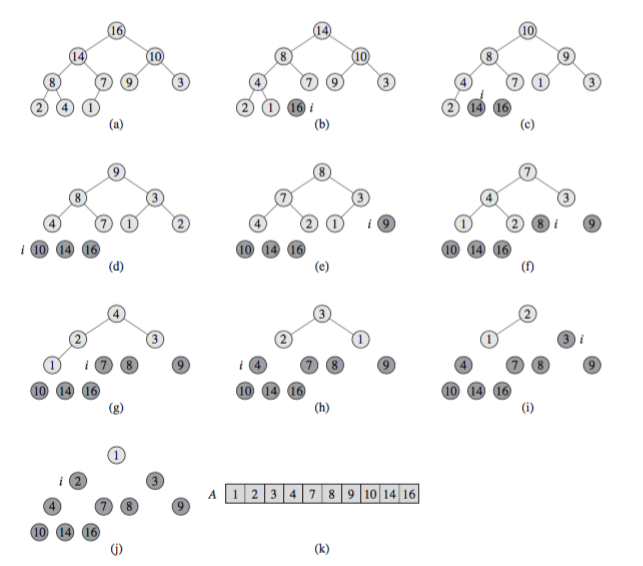
\includegraphics[width = 16.5cm, height = 10cm]{-1.png}
{\centering \linebreak \linebreak \small Figure 3.1.2: Operations of {\itshape Heap-Sort} algorithm. {\bfseries (a)} {\itshape Max-Heap} data structure after lines 30 - 31. {\bfseries (b)-(j)} The {\itshape max-heap} just after each call of {\itshape heapify} in line 37, showing the value of {\itshape i} at that time. Only lightly shaded nodes remain in the heap. {\bfseries (k)} Resulting sorted list.}
\end{figure}
